\documentclass[titlepage,12pt]{report}

\usepackage[utf8]{inputenc}
\usepackage[a4paper, total={6in, 8in},headheight=14pt]{geometry}
\usepackage{newtxtext,newtxmath}
\usepackage[scaled=1]{couriers}
\usepackage[spanish]{babel}
\usepackage{microtype}
\usepackage[bottom]{footmisc}
\usepackage{fancyhdr}
\usepackage{graphicx}
\usepackage{blindtext}
\usepackage{scrextend}
\usepackage{tocloft}
\usepackage{parskip}
\usepackage{multicol}
\usepackage{subcaption}
\usepackage{wrapfig}
\usepackage{multicol}
\usepackage{verbatimbox}
\usepackage[nottoc, notlot, notlof]{tocbibind}
\usepackage{listingsutf8}
\usepackage{url}
\usepackage[square,numbers]{natbib}
\usepackage{adjustbox}
\usepackage[makeroom]{cancel}
\usepackage[hidelinks]{hyperref}
\usepackage[Glenn]{fncychap}
\usepackage{lastpage}
\usepackage{fancyhdr}

\bibliographystyle{unsrtnat}

\pagestyle{fancy}
\fancyhf{}
\fancyhead[R]{\rightmark}
\fancyfoot[C]{\leftmark}
\fancyfoot[R]{\thepage}
\renewcommand{\footrulewidth}{0.6pt}% Line at the footer visible
\addto\captionscatalan{%
  \renewcommand\contentsname{Índice}%
}

\fancypagestyle{plain}{%
  \fancyhf{}%
  \fancyfoot[R]{\thepage}%
  \renewcommand{\headrulewidth}{0pt}% Line at the header invisible
  \renewcommand{\footrulewidth}{0.6pt}% Line at the footer visible
}


\renewcommand{\cftpartleader}{\cftdotfill{\cftdotsep}}%
\renewcommand{\cftsecleader}{\cftdotfill{\cftdotsep}}%
\renewcommand\familydefault{\sfdefault}

\usepackage{tikz}
\usetikzlibrary{shapes.geometric, arrows}

\newcommand{\Lagr}{\mathcal{L}}
\newcommand{\Xagr}{\mathcal{X}}

\setlength{\skip\footins}{1cm}

\makeatletter
% \patchcmd{<cmd>}{<search>}{<replace>}{<success>}{<failure>}
\patchcmd{\@makechapterhead}{\huge}{\large}{}{}% for \chapter
\patchcmd{\@makechapterhead}{\Huge}{\large}{}{}% for \chapter
\patchcmd{\@makeschapterhead}{\Huge}{\large}{}{}% for \chapter*
\makeatother


\begin{document}

\iftrue
\newcommand{\HRule}{\rule{\linewidth}{0.5mm}}

\thispagestyle{empty}

\begin{center}

{\large Universitat Politècnica de Catalunya}

\medskip
{\large Facultat d'Informàtica de Barcelona (FIB)}

\vfill
{\bfseries\Large Bachelor's Degree Project}

\vfill
\centerline{\mbox{
\includegraphics[width=60mm]{media/FIB_UPC.png}}}

\vfill
\vspace{5mm}

{\LARGE Jordi Gil González}

\vspace{15mm}

% Title in English according to the official assignment
{\LARGE\bfseries Analysis of the Path Tracing \\ rendering method on CPU and GPU}

\normalfont \small \sffamily{}

\vfill

Computer Science Department


\vfill

\begin{tabular}{rl}
Bachelor's Degree Project Director: & Chica Calaf, Antoni \\
\noalign{\vspace{2mm}}
Study programme: & Computer Science\\
\noalign{\vspace{2mm}}
Specialization: & Computer Graphics\\
\end{tabular}

\vfill

\large Academic Year 2019/2020

\large \today

\end{center}

\newpage
\tableofcontents*
\fi

\newpage

\chapter{Contextualización y alcance del proyecto}

\section{Introducción} \label{introduction}

En la actualidad, las imágenes generadas por ordenador están muy presentes tanto en el entorno profesional como en el lúdico. La creación de imágenes realistas mediante el uso de computadoras se ha convertido en una necesidad a la orden del día. Industrias como el cine o los videojuegos requieren de algoritmos capaces de reproducir el mundo real en un entorno virtual y, si siempre que se pueda, en el menor tiempo posible.

El estudio de métodos que permiten renderizar imágenes realistas no es nuevo. Entre principios y mediados de los años 70 comenzaron a publicarse los primeros artículos científicos en referencia a la simulación de la luz y el color sobre superficies modelos tridimensionales. Para poder entender como funcionan estos métodos debemos tener presente la representación de modelos 3D. 

Para representar un modelo 3D se utiliza una ''malla de polígonos'', popularmente conocida como \textit{Mesh} y generalmente estos polígonos suelen ser triángulos. Ésta consiste en un conjunto de vértices conectados por aristas formando caras. Para cada una de estas caras podemos definir un vector normal ortogonal a ésta.

Volviendo a los métodos de cálculo de iluminación, el más simple de todos es el conocido como \textit{Flat Shading}. Para calcular el color de cada una de las caras de nuestra malla solamente tiene en cuenta un vértice de los que la conforman y la normal de ésta, aunque una malla compuesta por triángulos es común utilizar el centroide. El color se interpola para todos los vértices de la cara utilizando el color calculado al inicio dando así un resultado uniforme para toda la cara. Debido a no tener en cuenta las caras adyacentes esto produce resultados diferentes entre ellas. En la Figura \ref{flat:shading} podemos observar el efecto generado por este método. Podríamos pensar que añadir más vértices a nuestra malla los resultados mejorarían, pero no es una propuesta adecuada debido al mayor uso de memoria requerido y el problema no quedaría resuelto. Si hiciéramos \textit{zoom in} en el modelo, volveríamos a apreciar el efecto conocido como ''bandas de Mach'' \citep{Lotto1999}.

\begin{figure}[ht]
	\centering
	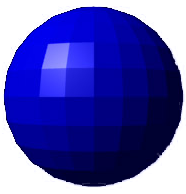
\includegraphics[scale=0.5]{media/Flat-shading-sample.png}
	\caption{Ejemplo de \textit{Flat Shading}. Fuente: Wikipedia}
	\label{flat:shading}
\end{figure}

En los métodos de sombreado suave (\textit{Smooth Shading}), el color cambia de pixel a pixel y no de cara a cara, resultando así en transiciones suaves entre las diferentes caras adyacentes.
En 1971 Henri Gouraud nos presenta en su artículo \textit{Continuous Shading of Curved Surfaces} \citep{Henri1971} el sombreado de Gouraud (\textit{Gouraud Shading}). Este método nos permite añadir mayor continuidad al sombreado respecto al método de \textit{Flat Shading}. El gran avance respecto al método presentado anteriormente es que no precisa de una malla de gran densidad para lograr simular una mayor continuidad. Para cada pixel se determina su intensidad por interpolación de las intensidades definidas en los vértices de cada polígono.

\begin{itemize}
	\item Para cada vértice se define una normal como promedio de las normales de los polígonos a los que pertenece dicho vértice.
	\item Mediante el uso de algún modelo de iluminación como, por ejemplo, el modelo de reflexión de Phong, se calcula la intensidad de cada vértice utilizando la normal obtenida en el punto anterior.
	\item Para cada pixel, se interpola la intensidad en los vértices para obtener la intensidad de éste.
\end{itemize} 

Como podemos observar en la Figura \ref{Gouraud:shading}, los resultados obtenidos respecto el método anterior son notablemente superiores, pero no acaba de representar de forma correcta los reflejos especulares. Éstos puede suponer un problema grave si se presentan en el centro de un polígono (cara) de gran tamaño.

\begin{figure}[ht]
	\centering
	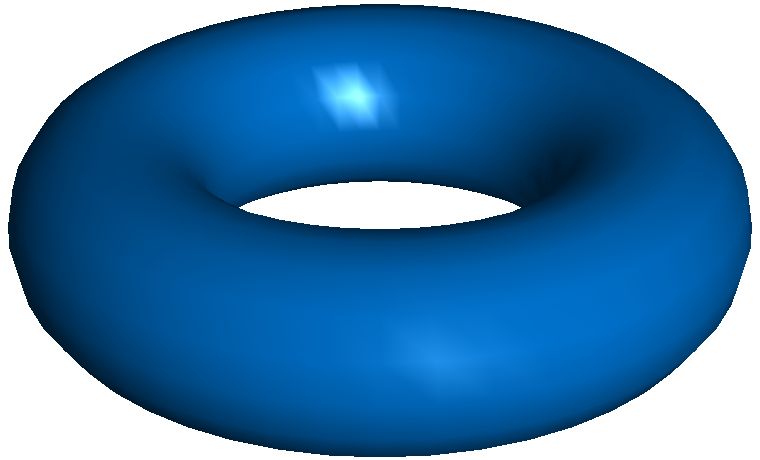
\includegraphics[scale=0.25]{media/Gouraudshading00.png}
	\caption{Ejemplo de \textit{Gouraud Shading}. Fuente: Wikipedia}
	\label{Gouraud:shading}
\end{figure}

Más tarde, Bui Tuong Phong en su tesis doctoral \citep{Phong1975} nos presentaba el sombreado de Phong. En el método presentado por Phong en vez de calcular la intensidad en el vértice, primero se define la normal de éste, se interpola y normaliza para cada pixel y es entonces cuando haciendo uso de algún modelo de iluminación se determina la intensidad final. El modelo resulta más costoso computacionalmente, debido a que el calculo se hace a nivel de fragmento (pixel) y no a nivel de vértice.

Phong menciona en su artículo publicado por la ACM \citep[p.~311]{Phong1975} que su objetivo no era simular la realidad, sino más bien añadir cierto grado de realismo:
\vspace{5mm}

\begin{mdframed}[hidealllines=true,backgroundcolor=gray!20] ''\textit{In trying to improve the quality of the synthetic images, we do not expect to be able to display the object exactly as it would appear in reality, with texture, overcast shadows, etc. We hope only to display an image that approximates the real object closely enough to provide a certain degree of realism.}'' 
\end{mdframed}

A pesar de que estos métodos supusieron, en lo concerniente al realismo, un avance, no pretenden simular la realidad. Además, éstos solamente tienen en cuenta la luz ambiente, difusa y especular. No tienen presente la iluminación indirecta de la escena, factor importante a la hora de crear imágenes que produzcan efectos realistas tales como, por ejemplo, reflejos.

No fue hasta los años 80 en que aparecieron los primeros métodos capaces de renderizar imágenes realistas. Turner Whitted nos presentaba en la sexta conferencia anual sobre \textit{Computer graphics and interactive techniques (SIGGRAPH)} el método de trazado de rayos, conocido popularmente por su nombre en inglés, \textit{Ray Tracing} \citep{Whitted1980}. Este método está basado en el algoritmo de \textit{Ray Casting}, presentado por Arthur Appel \citep{Appel1968}, consistente en trazar rayos desde el observador, uno por pixel, para determinar cual es el objeto más cercano. Además, una vez el rayo impacta en una superficie, basándonos en las propiedades de los materiales definidos en el objeto y las propiedades de la luz, se calcula el color. Se puede hacer uso de \textit{texture maps} para simular efectos como sombras. 

En 1986, David Immel et al. y James T. Kajiya, investigadores de la Cornell University y del California Institute of Technology (Caltech) respectivamente, presentaban de forma conjunta, en la décima tercera conferencia anual sobre \textit{Computer graphics and interactive techniques (SIGGRAPH)}, la \textit{Rendering Equation} \citep{Kajiya1986, Immel1986}. Dicha ecuación integral trata de resumir en una sola fórmula como la luz interactúa cuando impacta con una superficie haciendo uso de funciones probabilísticas llamadas "función de distribución de la reflectividad bidireccional", (BRDF por sus siglas en inglés). Ésta también tiene presente el ángulo en el que incide el rayo, la cantidad de fotones que llegan, los fotones emitidos desde otros puntos de la escena (iluminación indirecta), etc.

Otros métodos que nos permiten generar imágenes realistas a partir de calcular aproximaciones de la RE son: \textit{Bidirectional Path Tracing} presentado por \citep{Lafortune1993}, \textit{Photon Mapping} formulado por \citep{Jensen1996} y \textit{Metropolis light Transport} introducido por \citep{Veach1997}.

\section{Contextualización}

\subsection{Contexto} \label{ref:contexto}

Durante los estudios del grado, son varias las asignaturas dedicadas a la computación gráfica. En estas asignaturas se nos presentan los métodos de renderización realistas. Pero más allá de la introducción teórica a éstos, nunca se llegan a poner en práctica. De aquí nace la idea de realizar el presente proyecto, poder profundizar más en el tema de renderización realistas y así crear un aplicación en función a lo aprendido. Se pondrán también en práctica otros aspectos de la informática vistas en otras asignaturas como, por ejemplo, la creación de aplicaciones paralelas tanto en CPU como en GPU.

Como hemos indicado en la sección anterior, la renderización de imágenes realistas es un área de gran interés en el campo de la computación gráfica. Uno de los principales objetivos de ésta es ser capaces de renderizar imágenes indistinguibles de las del mundo real como, por ejemplo, fotografías. Siguiendo estas coordenadas, poder reproducir el comportamiento de la luz en un entorno virtual supone una tarea una importancia capital. Es primordial tener presente la iluminación global de una escena para poder obtener un alto grado de realismo. La iluminación global de una escena se compone de: \begin{enumerate*}[label=\roman*)] \item luz directa \label{item:dl}, \item luz indirecta \label{item:il} \end{enumerate*}.

\ref{item:dl} La luz directa es aquella que incide en un punto desde el foco de luz. \\
\ref{item:il} La luz indirecta es aquella que incide en un punto proveniente de la luz que rebota en otros puntos de la escena.

Recuperando lo expuesto en la introducción, el primer método capaz de renderizar imágenes realistas fue el \textit{Ray Tracing}, basado en la técnica de \textit{Ray Casting} de trazar rayos desde el observador a todos los pixeles de la imagen. La gran novedad respecto al algoritmo presentado por Appel \citep{Appel1968} es la incorporación de la recursividad. Cuando un rayo impacta contra un superficie puede generar tres tipos de rayos nuevos: \begin{enumerate*}[label=\roman*)] \item rayo de reflexión \label{ray:reflected}, \item rayo de refracción y \item rayo de sombra \end{enumerate*}. Al trazar los rayos nuevos somos capaces de conseguir efectos como reflejos, sombras, etc. debido a que para calcular el color estamos teniendo en cuenta como los demás objetos de la escena se afectan entre si. Una gran desventaja de este método es la dependencia que éste tiene respecto a los polígonos de la escena; a más compleja es, más ineficiente será. A pesar de ofrecernos un alto grado de realismo al ser capaz de tratar con precisión efectos ópticos como la refracción, reflexión, los resultados obtenidos en una imagen renderizada mediante \textit{Ray Tracing} no son necesariamente foto-realistas. Para conseguir renderizar imágenes foto-realistas debemos aproximar la RE, un buen ejemplo de ello es el método de \textit{Path Tracing} presentado por Kajiya \citep{Kajiya1986}.

El algoritmo de \textit{Path Tracing} surge como mejora del \textit{Ray Tracing} con el objetivo de dar una solución a la RE mediante la integración de Monte Carlo. Es gracias a ésto que el algoritmo es capaz, de forma natural, representar efectos como \textit{Motion Blur}, \textit{Ambient Oclussion} e iluminación indirecta sin necesidad de posprocesado. A diferencia del \textit{Ray Tracing}, el \textit{Path Tracing} es indiferente al número de polígonos presentes en la escena. Como hemos mencionado anteriormente, en el primer método se traza un rayo por cada polígono de la escena, en cambio en el método de Kajiya el rayo se traza por pixel. Debido a que cada uno es independiente de los demás, tenemos un algoritmo con una alta capacidad de paralelismo. En consecuencia, podemos explotar la capacidad de concurrencia que nos proporcionan las CPUs y GPUs; y poder así calcular más de un pixel de la imagen al mismo tiempo.

En este proyecto partiremos de la base de la implementación propuesta por Peter Shirley en su ''saga'' de libros sobre \textit{Ray Tracing} \citep{ShirleyRTOW, ShirleyRTNW, ShirleyRTL} para implementar nuestro \textit{Path Tracing}. La idea principal es desarrollar tres aplicaciones (una secuencia, una paralela en CPU y otra paralela en GPU) partiendo de la base que nos presenta Shirley, para poder hacer un análisis que como es el rendimiento de un \textit{Path Traing} explotando la capacidad de concurrencia de una CPU contra la de una GPU.

La forma en que representemos nuestra escena tendrá un gran impacto a la hora de calcular el color de la imagen final. Como hemos comentado, la base del método es trazar rayos por la escena para calcular el color de cada pixel. Si nuestra representación de la escena consiste en almacenar todos los objetos en una estructura de datos de tipo lista o vector ordenados por orden de creación, a la hora de calcular un punto de la imagen en el peor caso estaremos recorriendo todo el conjunto de polígonos de la escena para determinar el color final. Tratar de renderizar una escena que, muy posiblemente, esté compuesta de millones de polígonos puede traducirse en horas y horas de procesado. Es por eso que haremos uso de una estructura de datos aceleradora que nos permita representar la escena de una forma más inteligente, para que a la hora de determinar si un rayo impacta o no un polígono se determine de la forma más rápida posible.

\subsection{Stakeholders}

En esta sección presentaremos cuales son los diferentes actores implicados en un proyecto.

\subsubsection{Desarrollador}

Este actor es el encargado de realizar la planificación del proyecto, búsqueda de información, documentación, desarrollo del software requerido, solución de posibles obstáculos y/o problemas que puedan aparecer a lo largo del desarrollo y realización y análisis de los experimentos. Debe trabajar de forma conjunta y coordinada con el director, y co-director y/o ponente si lo hay, y es la última persona encargada del cumplimiento de los términos establecidos.

\subsubsection{Director del proyecto}

Este actor es el encargado de guiar al desarrollador en caso de dificultades, así como del asesoramiento de posibles soluciones.

\subsubsection{Usuarios beneficiados}

Aunque este proyecto no tiene la intención de crear un producto, no quiere decir que no existan beneficiarios. Explorar diferentes vías de optimización haciendo uso de arquitecturas paralelas puede ser útil para investigadores y desarrolladores en el campo de la computación gráfica.

\section{Justificación}

En la actualidad son muchas las librerías orientadas a la programación en GPU. Tenemos librerías como \texttt{OpenCL} y \texttt{OpenACC}, que nos permiten una mayor portabilidad entre tarjetas gráficas de distintos fabricantes como por ejemplo \texttt{AMD} y \texttt{NVIDIA}. Pero para este proyecto hemos decidido escoger el entorno de \texttt{CUDA} desarrollado por \texttt{NVIDIA} específicamente para sus tarjetas gráficas y aceleradores. Decidimos usar esta API debido a que se trata de software propietario, mejor optimizado para las tarjetas de dicha empresa como bien nos indican Kamran Karimi et. al. \citep{Karimi2010} y Jianbin Fang et. al. \citep{Fang2011} respectivamente en sus artículos científicos, las cuales utilizaremos en este proyecto.

Es posible que, citadas tarjetas/aceleradores \texttt{NVIDIA} y, teniendo presente que el proyecto está enfocado al tema de renderizado de gráficos realistas, al lector del presente Trabajo de Fin de Grado le venga a la mente la nueva gama de tarjetas RTX diseñada por \texttt{NVIDIA}. En un inicio se planteó guiar el proyecto hacia el uso de tarjetas con tecnología RTX debido a que éstas han sido diseñadas específicamente para el uso de \textit{Ray Tracing} en tiempo real. Esta idea fue descartada en seguida debido al elevado precio de éstas. El rango de precios de las tarjetas de esta gama oscila entre los 350€ en los modelos más económicos, hasta los varios miles de euros en modelos destinados a entornos profesionales. Finalmente, aunque el autor de dicho trabajo adquirió una tarjeta gráfica NVIDIA RTX 280 Super con 8Gb de memoria, se decidió no guiar el proyecto a utilizarla de forma exclusiva, estudiando y poniendo en práctica las nuevas mejoras que ésta ofrece (RT Cores, Tensor Cores, Mesh Shaders, etc.), frente a otras tarjetas de gamas inferiores que no incluyen, debido al corto plazo de tiempo para el desarrollo. Es por eso que esta tarjeta gráfica será usada para testar nuestra aplicación, pero no en un sentido exclusivo.

Como hemos comentado al inicio de esta sección, \texttt{CUDA} es un API que está muy bien optimizada para hardware de \texttt{NVIDIA}. Esto nos da un punto a favor debido a que la aplicación que vamos a desarrollar será probada en diferentes entornos que utilizan la tecnología de NVIDIA:

\begin{enumerate}
	\item Computador portátil - Lenovo Legion Y520 con Nvidia GTX1050 Mobile - 4GB.
	\item Computador personal - Nvidia RTX 2080 Super - 8Gb.
	\item Cluster docencia BOADA - 4 GPUs Nvidia Tesla K40c.
\end{enumerate}

Al usar tarjetas en entornos diferentes podremos analizar como nuestra aplicación responde en cada uno de ellos y estudiar así cómo es el rendimiento cuando utilizamos varias tarjetas pensadas para un entorno de investigación/profesional, en contraposición con otras dos pensadas para un uso más cotidiano. También podremos ver como es el rendimiento en una tarjeta gráfica de gama media (Nvidia GTX1050 Mobile) y una de gama alta (Nvidia RTX 2080 Super); y hacer así una comparativa entre ellas.

\section{Alcance del proyecto}

Para solucionar el problema presentado en nuestro proyecto necesitamos una aplicación que sea capaz de renderizar imágenes realistas. Como hemos comentado unas secciones más atrás, en \citep{ShirleyRTOW, ShirleyRTNW, ShirleyRTL} se nos presentan las bases para crear un \textit{Ray Tracing}. A partir de esta base extenderemos nuestra aplicación a una versión paralela haciendo uso de la CPU y otra haciendo uso de la GPU.

También, como hemos comentado en la sección sobre el contexto, el uso de estructuras de datos aceleradoras es un factor importante en este tipo de aplicaciones y se llevan estudiando durante muchos años (p.e. \citep{Rubin1980}) por parte de la comunidad científica. En este proyecto haremos uso de la \textit{Bounding Volume Hierarchy}, que se trata de una estructura de tipo árbol, ya sea binario o n-aria, en el cual cada hoja representa la caja delimitadora (\textit{Bounding Box}) de cada primitiva de la escena; y cada nodo intermedio representa la caja delimitadora de sus hijos. De este modo, estamos representando la escena como un conjunto de cajas que nos permitirá saber de forma eficiente si un rayo impacta o no con un polígono y con cual de todos los que componen la escena.

Existen muchas formas de construir un BVH, en nuestro caso nos hemos decantado por versión la presentada por Tero Karras \citep{Karras2012, Karras2013}. La forma en la que se construye el árbol nos permite explotar al máximo la concurrencia que nos proporciona la CPU y la GPU ya que es posible construir cada nodo del árbol de forma independiente. 

\subsection{Alcance}

En este apartado se presentan los diferentes objetivos y posibles obstáculos del proyecto.

\subsection{Objetivo}

Son varios los objetivos principales que nos proponemos en este proyecto. El primero se trata de desarrollar aplicación que dada una escena renderice una escena mediante el método \textit{Path Tracing} y analizar el rendimiento que éste nos ofrece en su versión paralela en CPU y en su versión en GPU.

Otro objetivo principal es estudiar y poner en práctica cuales son las mejores prácticas en la gestión de memoria en una aplicación paralela se refiere.

Como objetivos secundarios tenemos:

\begin{enumerate}
	\item Implementar de forma eficiente el método presentado por P. Shirley \citep{ShirleyRTOW, ShirleyRTNW, ShirleyRTL} y T. Karras \citep{Karras2012}.
	\item \label{ref:info} Buscar información sobre técnicas de optimización en el cálculo de intersección rayo-objeto.
	\item Implementar de forma eficiente los cálculos de intersección rayo-objeto.
	\item Extender la aplicación para renderizar modelos 3D.
\end{enumerate}

\subsection{Obstáculos y riesgos del proyecto}

Los temas principales en los que se centra el presente proyecto han sido muy estudiados por parte de la comunidad científica. No obstante, esto no implica que el desarrollo de éste sea una tarea sencilla, pues son muchos los problemas u obstáculos a los cuales podemos enfrentarnos.

\subsubsection{Programa principal}

Como bien hemos comentado en la sección de objetivos, la gestión de memoria es un factor muy importante. Una mala gestión de ésta puede provocar errores que no permitan el correcto funcionamiento de la aplicación.

\subsubsection{Algoritmo utilizado}

El algoritmo utilizado calcula el color a partir de la intersección de los rayos emitidos desde la cámara a los diferentes pixeles de la escena. Al tratarse operaciones que se llevarán a cabo miles de millones de veces en la creación de una imagen, tener una mala implementación de éstas puede afectar al rendimiento de nuestra aplicación de forma negativa.

\section{Metodología y rigor}

En esta sección veremos el conjunto de herramientas que se usarán a lo largo del desarrollo del presente proyecto. Para poder llevar un buen desarrollo de éste nos organizaremos de la siguiente forma: \begin{enumerate*}[label=\roman*)] \item Reuniones cada 15 días con el director del presente proyecto para comentar el estado de éste, resultados obtenidos, carencias, objetivos cumplidos y no cumplidos y acordar los siguientes pasos a realizar. \item Reuniones semanales de cara a la fase final del desarrollo. \end{enumerate*}

\subsection{Metodología}

La metodología de trabajo que se seguirá en el presente proyecto es la conocida como \textit{agile}. Cada iteración del ciclo de vida corresponderá con el inicio de una reunión con el director del proyecto hasta el inicio de la siguiente. En cada reunión se especificará una serie de objetivos, que deberán cumplirse de cara a la siguiente vista y en la que se evaluarán cuales han sido cumplidos y cuales no.

\subsection{Herramientas de desarrollo}

El desarrollo de nuestra aplicación se llevará a cabo en C++ haciendo uso de las librerías \texttt{OpenMP} y \texttt{CUDA}. 

\texttt{OpenMP} es una API diseñada para añadir concurrencia a programas escritos en \texttt{C}, \texttt{C++} y \texttt{Fortran}. La principal ventaja de usar esta API, en contra de otras de características similares, es que nos permite escribir un código portable entre diferentes sistemas operativos como podría ser Linux, Windows o MAC y nos permite crear de forma sencilla aplicaciones paralelas haciendo uso de la CPU.

\texttt{CUDA} es una plataforma de computación paralela y una API desarrollada por \texttt{NVIDIA} que nos permite acceder al conjunto de instrucciones y elementos de cómputo de las tarjetas gráficas y aceleradores de \texttt{NVIDIA} para poder crear aplicaciones paralelas haciendo uso de la GPU.

\subsection{Herramientas de seguimiento}

Por tal de llevar a cabo un buen seguimiento del desarrollo del presente proyecto se hará uso de \texttt{git}. Esta herramienta nos permite llevar un control de versiones que nos permitirá consultar versiones anteriores de nuestro código en caso de ser necesario.

\newpage
\nocite{*}

\printbibliography

\end{document}
